%---Packages---%
\documentclass[a4paper,11pt]{article}
\usepackage[left=2.5cm,top=2cm,right=2cm,nohead]{geometry}
\usepackage[french]{babel}
\usepackage[T1]{fontenc}
\usepackage[utf8]{inputenc} 
\usepackage{graphicx}
\usepackage{float}
\usepackage{amsmath}
\usepackage{amsfonts}
\usepackage{amssymb}
\usepackage{listings}
\usepackage{mdwlist}
\usepackage[usenames,dvipsnames]{color}
\usepackage[stable]{footmisc}%To include footnotes in 'section' parts
\usepackage{hyperref}
\usepackage{setspace}
\usepackage{eurosym}
\usepackage[section]{algorithm} % [section] is use to define the numbering mode
\usepackage{algorithmic} 

%---Insertion de code---%
\definecolor{lightgray}{gray}{0.95}


\lstset
{           
backgroundcolor=\color{lightgray},
keywordstyle=\color{Red}\bfseries,
ndkeywordstyle=\color{darkgray}\bfseries,
commentstyle=\color{Green},
stringstyle=\color{Orange},
basicstyle=\footnotesize,       % the size of the fonts that are used for the code
numbers=left,                   % where to put the line-numbers
numberstyle=\footnotesize,      % the size of the fonts that are used for the line-numbers
stepnumber=2,                   % the step between two line-numbers. If it's 1 each line will be numbered 
numbersep=5pt,                  % how far the line-numbers are from the code
showspaces=false,               % show spaces adding particular underscores
showstringspaces=false,         % underline spaces within strings
showtabs=false,                 % show tabs within strings adding particular underscores
tabsize=2,	                % sets default tabsize to 2 spaces
captionpos=b,                   % sets the caption-position to bottom
breaklines=true,                % sets automatic line breaking
breakatwhitespace=false,        % sets if automatic breaks should only happen at whitespace
title=\lstname,                 % show the filename of files included with \lstinputlisting & 
escapeinside={\%*}{*)},         % if you want to add a comment within your code
morekeywords={*,...}            % if you want to add more keywords to the set
extendedchars=true
}

%---Liens---%
\hypersetup{
unicode=false,          % non-Latin characters in Acrobat’s bookmarks
pdftoolbar=true,        % show Acrobat’s toolbar?
pdfmenubar=true,        % show Acrobat’s menu?
pdffitwindow=false,     % window fit to page when opened
pdfstartview={FitH},    % fits the width of the page to the window
pdftitle={Projet AGGP - Synthèse des articles},    % title
pdfauthor={Balthazar Rouberol, Anthony Tschirhard, Marion Poirel, Marie Paturel},     % author
pdfsubject={Projet AGGP - Dossier d'init},   % subject of the document
pdfcreator={Balthazar Rouberol, Anthony Tschirhard, Marion Poirel, Marie Paturel},   % creator of the document
pdfkeywords={Réseaux biologiques, Réseaux, AlgoGen}, % list of keywords
pdfnewwindow=true,      % links in new window
colorlinks=true,       % false: boxed links; true: colored links
linkcolor=black,          % color of internal links
citecolor=black,        % color of links to bibliography
filecolor=white,      % color of file links
urlcolor= NavyBlue,           % color of external links
bookmarks=true,% show bookmarks bar?
bookmarksopen=false,
bookmarksnumbered = false      
}%



\begin{document}
\maketitle

L'objectif de ce document est de prévoir la conception du projet en explicitant l'organisation du code ainsi que le planning des phases de codage, de tests et d'exploitation du code. Ainsi, sa lecture devrait permettre de connaître précisément la division du projet, à la fois au niveau humain (organisation au sein de l'équipe) et temporel.

%%%%%%%%%%%%%%%%%%%%%%%%%%%%%%%%%%%%%%%%%
\section{Présentation générale du projet}

\subsection{Algorithme génétique}
Le but de ce projet est de faire évoluer une population de réseaux grâce à un algorithme génétique pré-existant. Nous devons définir une \textit{fitness} qui permet de sélectionner les individus sur leurs capacités à s'approcher d'un réseau biologique.

Un individu correspondant à un réseau, le génome manipulé par l'algorithme génétique est une concaténation des lignes de la partie triangulaire supérieure de la matrice d'adjacence du réseau. Celle-ci étant ici symétrique, le réseau est ainsi parfaitement représenté.

\subsection{Livrables et délais}
Nous devons produire un réseau respectant les propriétés d'un réseau biologique, et pouvoir le présenter pour le mercredi 13 avril, c'est à dire 5 semaines après le début du projet.

\subsection{L'équipe}
\begin{itemize}
\item Chef de Projet : Balthazar Rouberol
\item Responsable Qualité : Marion Poirel
\item Ma\^itre d'œuvre : Anthony Tschirhard
\item Responsable Documentation : Marie Paturel
\item Groupe d'étude informatique : Balthazar Rouberol, Anthony Tschirhard, Marion Poirel, Marie Paturel
\end{itemize}



%%%%%%%%%%%%%%%%%%%%%%%%%%%%%%%%%%%%%%%%%%%%%%%%%%%%%%%%%%
\section{Rappel sur les réseaux biologiques}
% Anthony

Rappellons ici les propriétés générales d'un réseau biologique à valider par les réseaux à générer :
\begin{itemize}
	\item la répartition de ses degrés devra suivre une loi de puissance $ P(k) ~ \alpha k^{-\gamma} $, traduisant la faible présence de noeuds ultraconnectés : les hubs
	\item validation de la propriété de \og petit monde\fg
	\item formation de cliques 
\end{itemize}

\paragraph*{Paramètres de la loi de puissance\\}
La bibiographie suggère de fixer $\gamma $ entre 2 et 3 \footnote{Network biology : Understanding the cell's functional organization - A. Barbab\'{a}si \& Z. Oltvai - Nature reviews - Genetics - Feb 2004} ou de le fixer à 2.1\footnote{Exploring complex networks - S. Strogatz - Nature Vol 410 - March 2001}. Comme visible sur la figure \ref{scalefree}, la différence de distribution est relativement faible. Nous décidons donc de fixer $\gamma$ à $2.1$.


\paragraph*{Propriété de petit monde \\}
Cette propriété traduit le fait que tous les noeuds d'un graphe sont reliés. La valeur de la longueur de moyenne entre les noeuds dans un réseau métabolique est comprise entre 3 et 4\footnote{Network biology : Understanding the cell's functional organization - A. Barbab\'{a}si \& Z. Oltvai - Nature reviews - Genetics - Feb 2004}. Nous décidons donc de conserver cette condition et de l'appliquer aux réseaux générés.

\begin{wrapfigure}{r}{0.45\textwidth}
  %\vspace{200pt}
  \begin{center}
    \includegraphics[width=0.50\textwidth]{plot.png}
  \end{center}
  \caption{Distribution puissances limites}
  \label{scalefree}
\end{wrapfigure}
\paragraph*{Formation de cliques\\}

Un graphe compte un certain nombre de \textbf{cliques} de différentes tailles. Une clique est un ensemble de nœuds entièrement interconnectés. Le \textbf{coefficient de clustering} est un bon indicateur de la présence de cliques et se calcule pour chaque nœud de la manière suivante :
$$ C_i = \frac{2Ei}{k_i k_{i-1}} $$
avec
\begin{itemize}
 \item $E_i$ : nombre de liens entre voisins ;
 \item $k_i$ : nombre de voisins de $i$.
\end{itemize}
Nous allons utiliser le coefficient de \textit{clustering} global, c'est à dire la moyenne des coefficients de chaque nœud. Ainsi, nous aurons une valeur comprise entre $0$ et $1$ que nous pourrons utiliser dans notre fonction de \textit{fitness}.


%%%%%%%%%%%%%%%%%%%%%%%%
\section{Implémentation}
% Anthony

\subsection{Classes et objets}
% Anthony
\begin{figure}
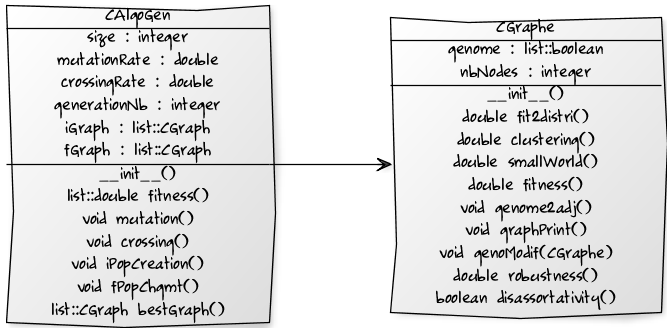
\includegraphics[width=\linewidth]{diagramme}
\caption{Diagramme de classe}
\label{diag}
\end{figure}
Comme le montre la figure~\ref{diag}, notre programme se compose de 2~classes principales : la classe \textbf{CGraph} et la classe \textbf{CAlgoGen}.

\subsection{Codage d'un réseau}
% Anthony
\subsubsection{Matrice d'adjacence}
Afin de coder nos réseaux, nous allons nous servir d'une \textit{matrice d'adjacence} : c'est une matrice de dimension $n * n$ dont l'élément non-diagonal $a_{ij}$ est le nombre d'arêtes liant le sommet $i$ au sommet $j$. L'élément diagonal $a_{ii}$ est le nombre de boucles au sommet $i$.

Notre graphe est simplifié :
\begin{itemize}
 \item graphe non orienté, \textit{ie.} notre matrice est diagonale ($\forall i, a_{ij}=a_{ji}$).
 \item absence de boucle aux sommets, \textit{ie.} la diagonale est nulle ($\forall i, a_{ii}=0$)
\end{itemize}

Nous n'allons donc garder que la partie triangulaire supérieure de notre matrice d'adjacence. Cela permettra de stocker moitié moins de données.

\subsubsection{Remplissage de la matrice}
La matrice peut être générée, par \verb?NetworkX? de deux manières : soit de manière aléatoire, soit de manière "biaisée", en influençant par exemple la répartition des degrés dans le graphe de départ. En effet, on veut converger vers nos trois critères de \textit{fitness} mais ceux-ci ne sont pas tous aussi simples à atteindre. Il est par exemple assez simple de converger vers la petit monde alors que converger vers la répartition des degrés voulue est plus long.

Nous avons donc décidé de partir d'un réseau dont la répartition des degrés de départ est biaisée et suit une loi exponentielle -- celle voulue.


\subsubsection{Fonctions}

\paragraph*{}

\subsection{Algorithme génétique}
%Afin de minimiser le temps de convergence, nous partons d'une distribution biaisée : la matrice est remplie selon une loi de puissance.
%
%On considère qu'un réseau est biologique s'il possède les trois propriétés suivantes :
%\begin{itemize}
%\item distribution des degrés selon une loi exponentielle de paramètre $2.2$\footnote{article ?} ,
%\item "petit monde",
%\item présence de cliques.
%\end{itemize} 
%
%A chaque génération, on vérifie l'adéquation de chaque réseau avec ses caractéristiques : leur somme pondérée définit la \textit{fitness} d'un individu. Les individus sont classés en fonction de leur \textit{fitness} et sélectionnés selon le procédure suivante : ???. Ceux conservés pour la nouvelle génération subissent des mutations, des \textit{crossing-over} (et des croisements ?), étapes fondamentales de l'évolution.
%
%Une fois la génération finale obtenue, on teste la robustesse des réseaux (conservation des propriétés malgré la suppression au hasard d'un nœud) ainsi que leur concordance avec la disassortativité (les hubs ne sont pas reliés entre eux).\\
%
%Cette simulation est faite plusieurs fois, sur X pas de temps (temps moyen de convergence, explication ?). Les paramètres finaux des réseaux sont conservés afin de permettre un étude comparative. D'un simulation à une autre, la pondération des paramètres de la loi de \textit{fitness} et le degré de la loi de puissance pourront varier, ce qui permet d'étudier leur impact respectif.

\subsection{Fonction de \textit{fitness} }
%Combinaison libéaire de fonction
%Pourquoi pondérer ?

%%%%%%%%%%%%%%%%%%%%%%%%%%%%%%%%%%%%%%%%%
\section{Planning}
\subsection{Répartition du code}

\subsection{Répartition du travail}

\begin{center}
\begin{table}[!h]
\begin{tabular}{|c|c|c|}
\hline Fonction & Attribué à & Date de rendu \\
\hline
Adaptation de \verb?AlgoGen? & Marie & 03/04 \\
\hline
\verb?fit2distri()? & Balthazar & 31/03 \\
\hline
\verb?clustering()? & Marie & 01/04\\
\hline 
\verb?smallWorld()? & Marion & 01/04\\
\hline
\verb?fitness()? & Anthony & 03/04\\
\hline 
\verb?genome2adj()? & Balthazar & 31/03 \\
\hline 
\verb?graphPrint()? & Balthazar & 01/04 \\
\hline 
\verb?genoModif()? & Anthony & 03/04 \\
\hline 
\verb?robustness()? & Marion & 05/04 \\
\hline 
\verb?dissasortativity()? & Marion & 05/04\\
\hline 
\end{tabular}
\end{table}
\end{center}

Chacun est responsable de tester les fonctions qui lui sont attribuées avant la date de rendu. Ces tests se feront sur des graphes créés avec \verb?NetworX? (manuellement et de façon automatique : scale-free, aléatoire, etc. ) et des données biologiques.

\subsection{Exploitation}

\subsection{Risques}


\end{document}